% assignment_3.tex
% CS 8735 - Unsupervised Learning (Fall 2015)
%     University of Missouri-Columbia
%             Chanmann Lim
%            October 2015

\documentclass[a4paper]{article}

\usepackage[margin=1 in]{geometry}
\usepackage{listings}
\usepackage{amsmath}
\usepackage{graphicx}
\usepackage{float}
\usepackage{multirow}

\everymath{\displaystyle}
\DeclareMathOperator*{\argmax}{\arg\!\max}
\DeclareMathOperator*{\argmin}{\arg\!\min}

\begin{document}
\setcounter{page}{6}

\noindent The Matlab code for all experiments is in the \textbf{Appendix} section.

\paragraph{4.1.} In this task, we are performing fuzzy c-means clustering with the fuzzifier parameter $q=2$ and distance measure $d(x_i, \theta_j) = (x_i-\theta_j)^TA(x_i-\theta_j)$ with $A=\mathbf{I}$ on GMD dataset from the homework 1 and by considering that there are four significant clusters $m=4$ represented by centroid or mean center.\\

	We randomly initialize the four clusters centroid using uniformly distribution random generator which gives the value between 0 and 1 then we got:

	\begin{align}
		\Theta^{(0)} &= [\theta_1^{(0)} \; \theta_2^{(0)} \; \theta_3^{(0)} \; \theta_4^{(0)}]; \\
			&= \begin{bmatrix}
				0.7802  &  0.6079  &  0.1048  &  0.5495 \\
    			0.3376  &  0.7413  &  0.1279  &  0.4852
			\end{bmatrix}
	\end{align}

	In the fuzzy c-means algorithm, we need to first compute $U = [u_{ij}]$ matrix where

	\begin{align}
		u_{ij} &= u_j(x_i) \\
			&= \frac{1}{\sum_{k=1}^m (\frac{d(x_i,\theta_j)}{d(x_i,\theta_k)})^{\frac{1}{q-1}}}
	\end{align}

	then updating the parameter $\theta_j$ by solving $\sum_{i=1}^N u_{ij}^q \frac{\partial d(x_i,\theta_j)}{\partial \theta_j} = 0$ and we obtain:

	\begin{equation}
		\theta_j = \frac{\sum_{i=1}^N u_{ij}^qx_i}{\sum_{i=1}^N u_{ij}^q}
	\end{equation}

	We repeat this process until the termination criterion $||\Theta(t)-\Theta(t-1)|| < \epsilon$ where $\epsilon = 0.001$ is met and the final values of $\Theta$ (cluster centroids) is:

	\begin{equation}
		\Theta = \begin{bmatrix}
					13.2092  &  0.8970  &  8.5777  &  4.5329 \\
    				2.8618  &  1.7325  &  6.4067  &  6.7135
				\end{bmatrix}
	\end{equation}

\paragraph{4.2.} With the estimated cluster centroids we can perform cluster assignment by assigning each samples to the closest cluster.

\begin{equation}
	j_n^* = \argmin_j d(x_n, \theta_j)
\end{equation}

	\begin{figure}[H]
		\centering
			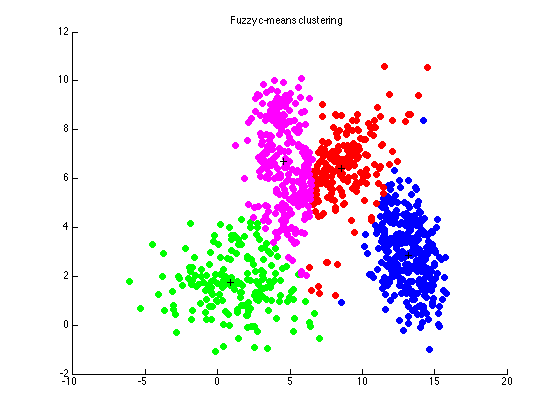
\includegraphics[scale=.54]{images/clusters_plot.png}
		\caption{Plot of samples for different clusters}
	\end{figure}

\paragraph{4.3.} Finally, we computed the total distortion for each iteration.

	\begin{equation}
		D(i) = \sum_{n=1}^N \min_j d(x_n, \theta_j(i))
	\end{equation}
	
	\begin{center}
		\begin{tabular}{ |c |c |c |c |c |c |c |c |c |c |c| }
			\hline
			i & 1 & 2 & 3 & 4 & 5 & 6 & 7 & 8 & 9 & 10 \\ \hline
			$D(i)$ & 27360 & 24016 & 17841 & 11821 & 9014 & 7400 & 5820 & 4925 & 4709 & 4683 \\ \hline
		\end{tabular}
	\end{center}
	
	\begin{center}
		\begin{tabular}{ |c |c |c |c |c |c |c |c |c |c |c| }
			\hline
			i & 11 & 12 & 13 & 14 & 15 & 16 & 17 & 18 & 19 & 20 \\ \hline
			$D(i)$ & 4689 & 4696 & 4700 & 4704 & 4706 & 4708 & 4709 & 4710 & 4711 & 4712 \\ \hline
		\end{tabular}
	\end{center}
	
	\begin{center}
		\begin{tabular}{ |c |c |c |c |c |c |c |c |c |c| }
			\hline
			i & 21 & 22 & 23 & 24 & 25 & 26 & 27 & 28 & 29 \\ \hline
			$D(i)$ & 4712 & 4713 & 4713 & 4713 & 4714 & 4714 & 4714 & 4714 & 4714 \\ \hline
		\end{tabular}
	\end{center}

	\begin{figure}[H]
		\centering
			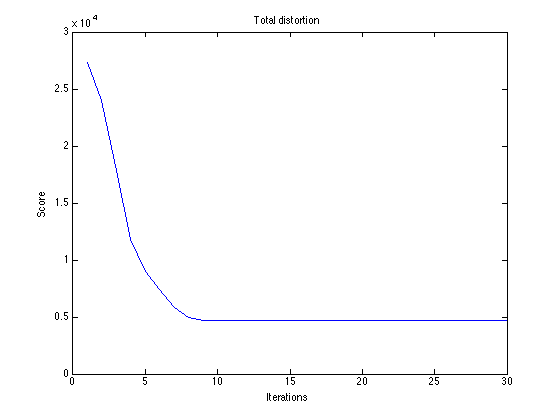
\includegraphics[scale=.55]{images/total_distortion.png}
		\caption{Total distortion}
	\end{figure}
	
	In this case we observed that there are slightly increase in total distortion scores from the 11\textsuperscript{th} iteration which is not the case in k-means clustering since fuzzy c-means clustering embraces the fuzzy nature to consider a vector belongs simultaneously to more than one clusters and the objective function $J_q(\theta, U)$ contains the weight $u_{ij}$ which balances the minimization.
	
	\begin{equation}
		J_q(\theta, U) = \sum_{i=1}^N \sum_{j=1}^m u_{ij}^q d(x_i, \theta_j)
	\end{equation}
	
\paragraph{5.} In this problem, we are working \textbf{GKlines.dat} dataset to perform Gustafson-Kessel clustering and we will let it run for five iterations. The merit that Gustafson-Kessel clustering brings is the incorporation of covariance matrix to better capture the shape of the planar cluster that can overcome collinear distinct cluster clustering issue in fuzzy c-varieties (FCV) algorithm. The distance measure for Gustafson-Kessel algorithm is defined as:

	\begin{equation}
		d^2_{GK}(x,\theta_j) = |\Sigma_j|^{1/l} (x-c_j)^T \Sigma_j^{-1} (x-c_j)
	\end{equation}
	
	By minimizing $J_{GK}(\theta, U) = \sum_{i=1}^N \sum_{j=1}^m u_{ij}^q d^2_{GK}(x_i,\theta_j)$ with respect to $c_j$ and $\theta_j$ we obtain:
	
	\begin{equation}
		c_j = \frac{\sum_{i=1}^N u^q_{ij}x_i}{\sum_{i=1}^N u^q_{ij}x}
	\end{equation}
	
	and
	
	\begin{equation}
		\Sigma_j = \frac{\sum_{i=1}^N u^q_{ij}(x-c_j)(x-c_j)^T}{\sum_{i=1}^N u^q_{ij}x}
	\end{equation}
	
\paragraph{5.2.b} The estimated cluster representatives $\theta(5)$:
	
	\begin{align}
		c^{(5)} &= [c_1^{(5)} \quad c_2^{(5)}]; \\
			&= \begin{bmatrix}
				-0.9964  &  0.2988 \\
    			 0.6515  &  0.7042
			\end{bmatrix}
	\end{align}
	
	\begin{align}
		\Sigma^{(5)} &= [\Sigma_1^{(5)} \Sigma_2^{(5)}]; \\
			&= \begin{bmatrix}
				0.0010  &  2.0179 \\
    			0.0060  & -2.0293 \\
    			2.0895  &  2.0426
			\end{bmatrix}
	\end{align}
	
	Where, $\Sigma_j$ is the upper triangular values for covariance matrix of the j\textsuperscript{th} cluster.
	
\paragraph{5.2.c} By using the parameters estimated from the first iteration we assigned each sample to clusters using minimum distance rule.

	\begin{equation}
		j^* = \argmin_j d^2_{GK}(x_n, \theta_j(1))
	\end{equation}

	\begin{figure}[H]
		\centering
			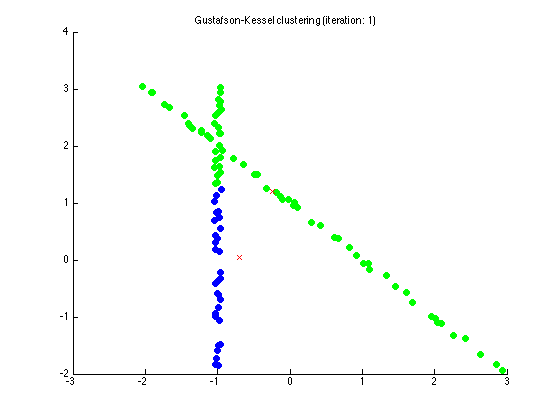
\includegraphics[scale=.55]{images/gk_clustering_1.png}
		\caption{Plot of samples in first iteration}
	\end{figure}

\paragraph{5.2.d} By using the parameters estimated from the fifth iteration.

	\begin{equation}
		j^* = \argmin_j d^2_{GK}(x_n, \theta_j(5))
	\end{equation}

	\begin{figure}[H]
		\centering
			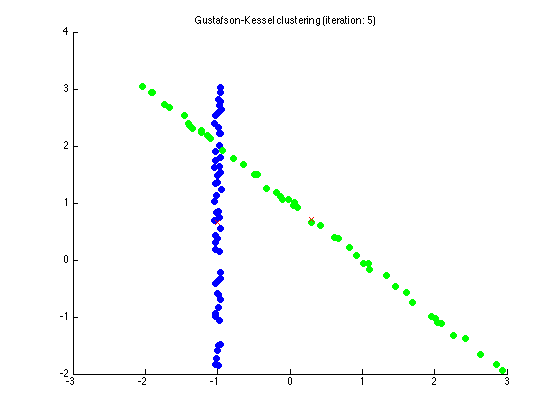
\includegraphics[scale=.55]{images/gk_clustering_5.png}
		\caption{Plot of samples in first iteration}
	\end{figure}
	
\paragraph{5.2.e} Finally, we computed the total distance in G-K clustering for each iteration.

	\begin{equation}
		D(i) = \sum_{n=1}^N \min_j d^2_{GK}(x_n, \theta_j(i))
	\end{equation}
	
	\begin{center}
		\begin{tabular}{ |c |c |c |c |c |c| }
			\hline
			i & 1 & 2 & 3 & 4 & 5 \\ \hline
			$D(i)$ & 107.2321 &  69.4622 &  38.1877  & 15.0506  &  9.3709 \\ \hline
		\end{tabular}
	\end{center}
		
\newpage
\subsection*{Appendix:}
	\lstinputlisting[language=Matlab, title=\lstname, basicstyle=\footnotesize]{assignment_3.m}
	\lstinputlisting[language=Matlab, title=\lstname, basicstyle=\footnotesize]{problem_3.m}
	\lstinputlisting[language=Matlab, title=\lstname, basicstyle=\footnotesize]{problem_4.m}
	\lstinputlisting[language=Matlab, title=\lstname, basicstyle=\footnotesize]{problem_5.m}
	\lstinputlisting[language=Matlab, title=\lstname, basicstyle=\footnotesize]{linkage.m}
	\lstinputlisting[language=Matlab, title=\lstname, basicstyle=\footnotesize]{vec2cell.m}
	\lstinputlisting[language=Matlab, title=\lstname, basicstyle=\footnotesize]{non_zero_min.m}
	\lstinputlisting[language=Matlab, title=\lstname, basicstyle=\footnotesize]{merge.m}
	\lstinputlisting[language=Matlab, title=\lstname, basicstyle=\footnotesize]{print_cluster.m}
	\lstinputlisting[language=Matlab, title=\lstname, basicstyle=\footnotesize]{fuzzy_c_mean.m}
	\lstinputlisting[language=Matlab, title=\lstname, basicstyle=\footnotesize]{point_distance.m}
	\lstinputlisting[language=Matlab, title=\lstname, basicstyle=\footnotesize]{total_distortion.m}
	\lstinputlisting[language=Matlab, title=\lstname, basicstyle=\footnotesize]{fcm_cluster_assignment.m}
	\lstinputlisting[language=Matlab, title=\lstname, basicstyle=\footnotesize]{sigma2vec.m}
	\lstinputlisting[language=Matlab, title=\lstname, basicstyle=\footnotesize]{vec2sigma.m}
	\lstinputlisting[language=Matlab, title=\lstname, basicstyle=\footnotesize]{gustafson_kessel.m}
	\lstinputlisting[language=Matlab, title=\lstname, basicstyle=\footnotesize]{gk_distance.m}
	\lstinputlisting[language=Matlab, title=\lstname, basicstyle=\footnotesize]{gk_total_distance.m}
	\lstinputlisting[language=Matlab, title=\lstname, basicstyle=\footnotesize]{gk_cluster_assignment.m}
\end{document}